\documentclass[9pt]{article}
\usepackage{ngerman}
\usepackage[utf8]{inputenc}
\usepackage{amsmath}
\usepackage{amsthm}
\usepackage{amssymb}
\usepackage{amsfonts}
\usepackage{mathrsfs}
\usepackage{stmaryrd}
\usepackage{enumerate}
\usepackage{listings}
\usepackage{color}
\usepackage{float}
\usepackage{mathtools}
\usepackage{fontawesome}
\usepackage{csquotes}
\usepackage{gensymb}
\usepackage{tikz}
\usepackage[margin = 2cm]{geometry}
\usepackage{verbatim}
\usepackage{hyperref}
\usetikzlibrary{calc}



\author{Niklas Schneider - Maximilian Krahn}
\date{}

\newcommand{\setFW}{
	\lstset{ %this is the stype
    mathescape=true,
    %frame=tB,				
    %numbers=left,
    %numberstyle=\tiny,		
    basicstyle=\ttfamily,
    keywordstyle=\color{blue}\bf,
    resetmargins=true,
    language = python,
    %xleftmargin=.04\textwidth,
    numbersep=0pt,
    tabsize=4
}
}
\lstnewenvironment{code}
{
	\setFW
}
{}

\lstMakeShortInline[
mathescape=true,
%frame=tB,				
%numbers=left,
%numberstyle=\tiny,		
basicstyle=\ttfamily,
keywordstyle=\color{blue}\bf,
resetmargins=true,
language = python,
%xleftmargin=.04\textwidth,
numbersep=0pt,
tabsize=4]@


\title{CoderDojo Saar - Turtle\\\textbf{Cheat Sheet}}

\begin{document}
    \maketitle
   
    \begin{center}
        \vspace{-1.5em}
        05.03. - 06.03.2021
        \rule{\textwidth}{1pt}
    \end{center}
  
    \subsection*{Python-Befehle}
    \subsubsection*{Variablen zuweisen}
    Um eine Variable in Python zuzuweisen, schreibst du einfach 
    zuerst den Namen der Variablen, dann ein @=@ und zuletzt den zugewiesenen Wert. Zum Beispiel: @a = 3@. Dann hat @a@ danach den Wert @3@.
    
    \subsubsection*{Datentypen}
    \begin{itemize}
        \item 
        \textbf{Ganzen Zahlen: } 
        Ganzen Zahlen wie @1@, @2@ oder @-3@ können einfach aufgeschrieben werden.

        \item 
        \textbf{Rationale Zahlen: } 
        Bei Kommazahlen wie @3.14@ werden die Dezimalstellen mit einem Punkt, nicht mit Komma getrennt werden. 

        \item 
        \textbf{Wahrheitswerte: }
        Es gibt die beiden Wahrheitswerte @True@ (wahr) oder @False@ (falsch). 

        \item 
        \textbf{Listen: }
        Um einer Variablen mehrere Werte zuzuweisen, können Listen benutzt werden.\\
        @x = [1, 2, 3, 4, 5]@ ist eine Liste der Zahlen 1 bis 5. Dabei werden die Elemente von eckigen Klammern umgeben und mit Kommata getrennt.
        
        \item 
        \textbf{Strings: }
        Wörter oder Texte werden mit einem String dargestellt, der durch @'@ oder @"@ signalisiert wird: @'Das ist ein String'@
    \end{itemize}

    
    \subsubsection*{Operatoren}
    \begin{itemize}
        \item \textbf{Vergleiche: }
        Die Operatoren @<@, @>@, @>=@, @<=@, @==@ geben Warheitswerte zurück, also wird zum Beispiel @42 < 1337@ zu @True@. 
        \item \textbf{Arithmetik: }
        Die Operatoren @+@, @-@, @*@, @/@ verhalten sich wie die mathematischen Operatoren. 
    \end{itemize}
    
    \subsubsection*{Ausgabe}
    Um etwas in der Konsole auszugeben, benutze ein Print-Statement: @print('Hallo Welt!')@
 
    \subsubsection*{If-statement:} 
    \begin{itemize}
        \item
        \textbf{Struktur:}\\
        Wenn ein Stück Code nur unter einer bestimmten Bedingung ausgeführt werden soll, kommt dieser in einen @if@-Block. 
        Das sieht zum Beispiel so aus:
        \begin{code}
if a < b:
    print('a ist kleiner als b')
    print('Das passiert nicht immer.')
else:
    print('a ist nicht kleiner als b')
print('Weil das hier nicht eindgerueckt ist, passiert es immer.')
        \end{code}
        Wichtig hierbei ist die Einrückung. Diese bestimmt, zu welchem Block eine Zeile gehört. So kann auch wie oben mehr als eine Zeile unter der Bedingung im @if@-Block ausgeführt werden.
    
        \item 
        \textbf{Alternativen:}\\
        Wenn die Bedingung nicht erfüllt ist, springt das Programm in den @else@-Block, wenn es einen gibt. Alternativ kann mit @elif bedingung:@ ein neuer Block mit neuer Bedingung hinzugefügt werden. 
    
        \item 
        Bedingungen können mit den logischen Operatoren @and@, @or@ oder @not@ verbunden werden.
    \end{itemize}  
    
    \subsubsection*{Funktionen} 
    Funktionen sind Codestücke, die einen eigenen Namen bekommen, damit man sie von überall im Programm aufrufen kann. 

    \begin{code}
def funktionsname(parameter_1, parameter_2):
    print('Das ist Parameter 1:' + str(parameter_1) + '\n')
    print('Das ist Parameter 2:' + str(parameter_2))
    \end{code}

    Funktionen, die einen Wert berechnen können diesen auch mit @return@ zurückgeben:
    \begin{code}
def summe(a, b):
    return a + b

print(summe(3, 4))
>>> 7
    \end{code}
        



    \subsection*{Turtle-Befehle}    
    Um die unten genannten Befehle zu verwenden, muss das Modul @turtle@ in der ersten Zeile mit @from turtle import *@ eingebunden sein. Das sollte in den vorgegebenen Dateien schon vorgegeben sein.
    \subsubsection*{Bewegen}
    \begin{itemize}
        \item 
        @forward(l)@\\
        Bewegt die Turtle um @l@ Einheiten in die aktuelle Blickrichtung nach vorne.
        \begin{figure}[H]
            \centering
            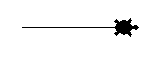
\includegraphics[scale = 0.8]{img/forward}
        \end{figure}
        
        \item 
        @back(l)@\\
        Bewegt die Turtle um @l@ Einheiten in die aktuelle Blickrichtung rückwärts.
        \begin{figure}[H]
            \centering
            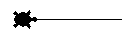
\includegraphics[scale = 0.8]{img/back}
        \end{figure}
    \end{itemize}

    \subsubsection*{Drehen}
    \begin{itemize}
        \item 
        @left(alpha)@\\
        Dreht die Turtle auf der Stelle um den Winkel @alpha@ nach links. Zum Beispiel für $30\degree$:
        \begin{figure}[H]
            \centering
            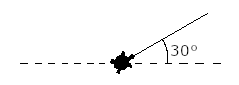
\includegraphics[scale = 0.8]{img/left}
        \end{figure}

        \item 
        @right(alpha)@\\
        Dreht die Turtle auf der Stelle um den Winkel @alpha@ nach rechts. Zum Beispiel für $30\degree$:
        \begin{figure}[H]
            \centering
            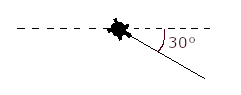
\includegraphics[scale = 0.8]{img/right}
        \end{figure}
    \end{itemize}
    
    \subsubsection*{Kreis}
    \begin{itemize}
        \item
        @circle(radius, alpha)@ \\
        Zeichnet einen Kreis mit dem Radius @radius@ und dem Winkel @alpha@ gegen den Uhrzeigersinn. Die Turle folgt dabei der
        Kreislinie und hat dadurch selbst den Winkel @alpha@. So ergibt zum Beispiel für @cicle(50,270)@: 
        \begin{center}
            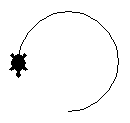
\includegraphics[scale = 0.8]{img/circle}
        \end{center}
    \end{itemize}

    \subsubsection*{Stift}
    \begin{itemize}
        \item 
        @color(farbe)@\\
        Setzt die Farbe des Stifts auf die angegebene @farbe@. Die @farbe@ ist ein Wert aus der folgenden Liste:
        \begin{center}
            @["red", "green", "blue", "white", "black", "yellow", "brown", "orange", "purple"]@
        \end{center}
        Weitere Farben findest du auf \url{https://matplotlib.org/stable/gallery/color/named_colors.html}
        
        \item 
        @bgcolor(farbe)@\\
        Setzt die Farbe der Leinwand auf die angegebene @farbe@. Es können dieselben Farben verwendet werden wie für @color(farbe)@.
        \item 
        @penup()@\\
        Lässt die Turtle ihren Stift hochheben. Alle nachfolgenden Bewegungen werden nicht mehr aufgezeichnet.
        
        \item 
        @pendown()@\\
        Lässt die Turtle ihren Stift wieder absetzen. Alle nachfolgenden Bewegungen werden wieder aufgezeichnet.
    \end{itemize}
    \begin{figure}[H]
        \centering
        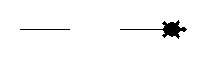
\includegraphics{img/pen}
    \end{figure}

    \subsubsection*{Allgemeines}
    \begin{itemize}
        \item 
        @pensize(dicke)@\\
        Stellt die Dicke des Stifts auf die gegebene @dicke@ ein. Die normale Einstellung der @dicke@ ist @1@. Als Dicke werden ganze und reelle Zahlen größer als 0 akzeptiert.

        \item 
        @speed(geschwindigkeit)@\\
        Stellt die Geschwindigkeit der Turtle auf die gegebene @geschwindigkeit@ ein. Die normale Einstellung der @geschwindigkeit@ ist @1@. 
        Je kleiner die Zahl ist, desto schneller wird die Turtle; dabei ist @0@ die schnellste Geschwindigkeit.
        Als Dicke werden ganze und reelle Zahlen größer oder gleich 0 akzeptiert.

        \item 
        @shape(form)@\\
        Stellt die Form der Turtle auf die gegebene @form@ ein. Möglich sind Werte aus der folgenden Liste:
        \begin{center}
            @["turtle", "classic", "arrow", "circle", "square", "triangle"]@
        \end{center}

        \item 
        @reset()@\\
        Setzt die Turtle wieder auf die Ausgangsposition zurück und löscht alle Zeichnungen.
    \end{itemize}
    
\end{document} 